Neben den beiden selbst erzeugten Szenarien, werden nun Szenarien betrachtet, in denen die Terrain-Generierung der Blocklib genutzt wird. Für die Generierung nutzt die Blocklib einen Pseudo-Zufallszahlengenerator. Das ist ein Algorithmus, der ausgehend von einem übergebenen Wert, dem sogenannten \emph{Seed} Werte erzeugt, die zufällig \emph{wirken}. Der Algorithmus ist allerdings deterministisch. Mit dem selben Seed wird immer die selbe Folge von Zahlen generiert.

\begin{figure}
	\centering
	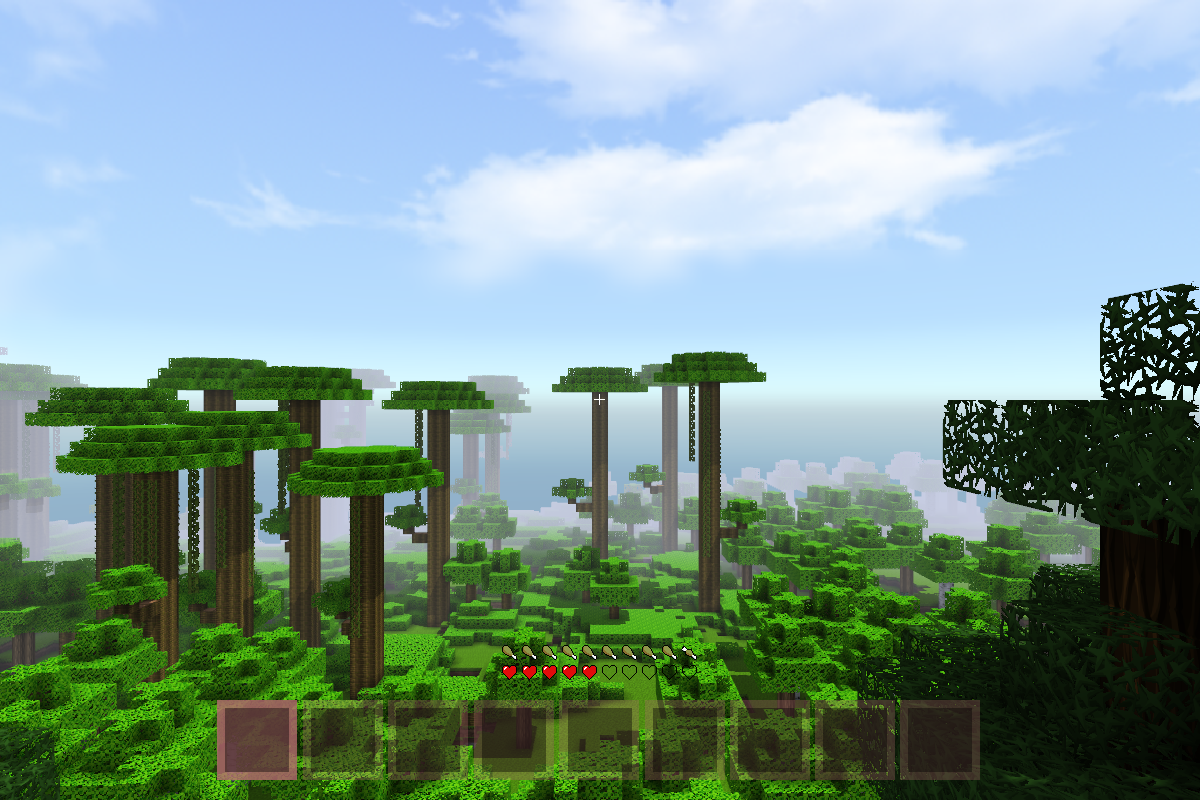
\includegraphics[width=.49\textwidth]{seed-0.png}
	\hfill
	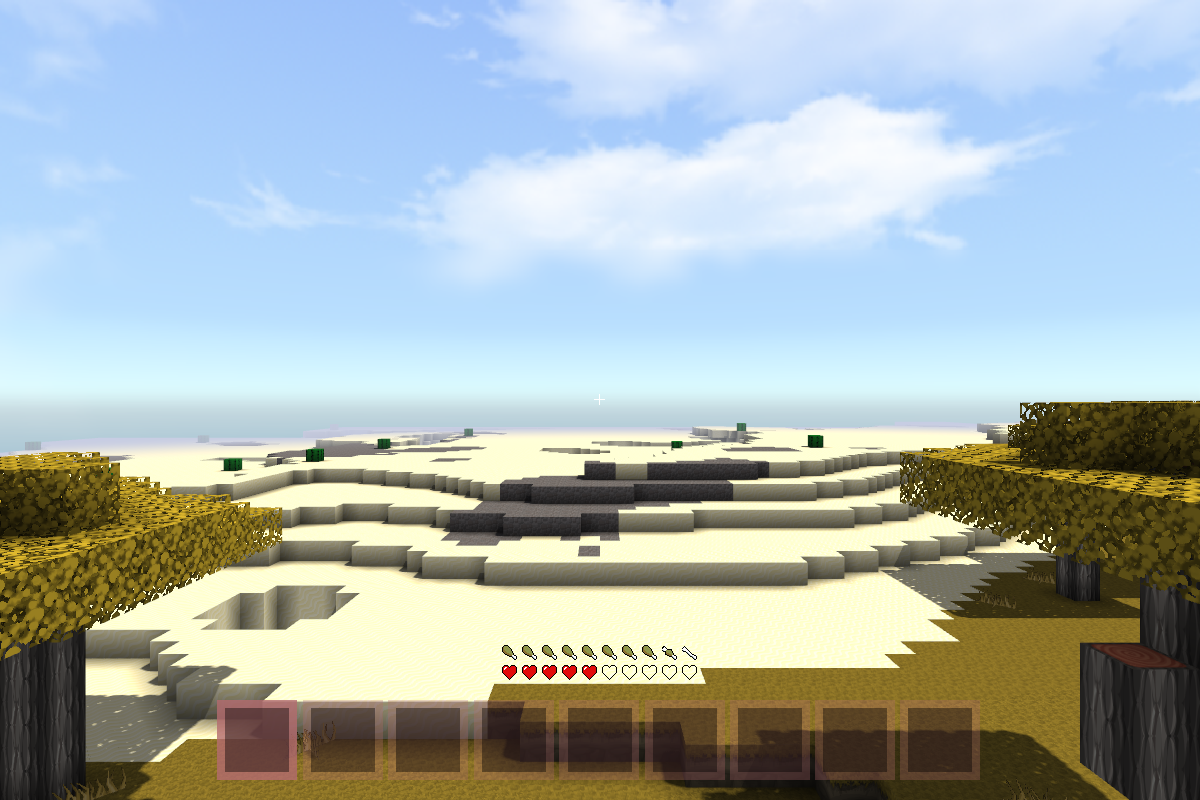
\includegraphics[width=.49\textwidth]{seed-2.png}
	\caption{Links: Seed 0. Rechts: Seed 2}\label{fig:static}
\end{figure}
Damit SystemA und SystemB bei Messungen mit Terrain-Generierung vergleichbar sind, wird in beiden Systemen der selbe Seed verwendet, wodurch die selbe Welt generiert wird. Abbildung~\ref{fig:static} zeigt zwei Screenshots von generierten Welten. Das linke Bild zeigt die mit dem Seed $0$ generierte Welt, das rechte Bild nutzt als Seed $2$. Hier sieht man beispielhaft, dass bereits kleine Unterschiede im Seed völlig andere Welten erzeugen. Für die folgenden Messungen wird der Seed $0$ verwendet. 

Im Szenario Welt Statisch wird bleibt die Kamera wie in den vorherigen beiden Szenarien an ein und der selben Stelle.



\paragraph{\ac{fps}}
\begin{figure}[!htbp]
	\fpsplot{seed-0-static}
	\caption{Seed 0 Statisch}\label{fig:seed-0-static-fps}
\end{figure}

\paragraph{CPU}
\begin{figure}[!htbp]
	\cpuplot{seed-0-static}
	\caption{Seed 0 Statisch}\label{fig:seed-0-static-cpu}
\end{figure}

\paragraph{GPU}
\begin{figure}[!htbp]
	\gpuplot{seed-0-static}
	\caption{Seed 0 Statisch}\label{fig:seed-0-static-gpu}
\end{figure}

\paragraph{RAM}
\begin{figure}[!htbp]
	\memplot{seed-0-static-single-mem.csv}
	\memplot{seed-0-static-multi-mem.csv}
	\caption{Seed 0 Statisch}\label{fig:seed-0-static-mem}
\end{figure} 
